\documentclass{beamer}
\usepackage[utf8]{inputenc}
\usepackage{amsmath, amsfonts, amssymb, amsthm}
\usepackage{array}
\usepackage{tikz}
\usetikzlibrary{positioning}
\usepackage{listings}
\usepackage{xcolor}
\usepackage{graphicx}

\definecolor{forestgreen}{RGB}{34, 139, 34}

\usetheme{Madrid}
\usecolortheme{default}

\graphicspath{{PICTURES/}}

\setbeamertemplate{footline}[frame number]
\setbeamertemplate{navigation symbols}{}

\title{Thue-Morse Sequence}
\author {Sava Darius-Ștefan}
\institute{Faculty of Computer Science\\University of Bucharest}
\date{27 May, 2025}

\begin{document}

\begin{frame}
    \titlepage
\end{frame}

\begin{frame}{Table of Contents}
    \tableofcontents
\end{frame}

\section{How to build this sequence}

\begin{frame}
    On Monday the baby said A, on Tuesday AU, on Wednesday AUUA, on Thursday AUUAUAAU. What will he say on Friday?

    \vspace{2cm}

    You can see that this very gifted baby increases her talking capacity twice each day. If the baby continues indefinitely, her text converges to an infinite sequence that mathematicians call the Thue-Morse sequence. Of course, mathematicians use zeroes and ones instead of A and U, so the sequence looks like 0110100110010110100 \dots
\end{frame}

\begin{frame}{Sequence construction}
    The Thue-Morse sequence, denoted as \( (t_n)_{n=0}^\infty \), can be constructed using the following methods:
    \vspace{1cm}
    \begin{enumerate}
        \item \textbf{Append the complement of the previous sequence:}\\
        Start with \( 0 \), and iteratively append the complement of the sequence generated so far:
        \[
        0, \quad 01, \quad 0110, \quad 01101001, \quad 0110100110010110, \dots
        \]
    \end{enumerate}
\end{frame}

\begin{frame}{Sequence Construction}
    \begin{enumerate}[2]
    \item \textbf{\large Lindenmayer system (L-system)}
    \end{enumerate}
    \vspace{0.5cm}
    Here is an alternate way to construct the sequence. In the same manner, we can start with $01$ and then we continually walk through the sequence, taking the next entry that we haven't visited yet (we consider that the first $0$ is visited), placing two copies at the end, and flipping the second bit. 

    \[
    01
    \]

    \[
        0 \rightarrow 0\textcolor{yellow}{0} \rightarrow 0\textcolor{yellow}{1} \hspace{3cm} 1 \rightarrow 1\textcolor{yellow}{1} \rightarrow 1\textcolor{yellow}{0}
    \]

\end{frame}

\begin{frame}{Sequence Construction}
    \begin{enumerate}[2]
    \item \textbf{\large Lindenmayer system (L-system)}
    \end{enumerate}
    \vspace{0.5cm}
    Here is an alternate way to construct the sequence. In the same manner, we can start with $01$ and then we continually walk through the sequence, taking the next entry that we haven't visited yet (we consider that the first $0$ is visited), placing two copies at the end, and flipping the second bit. 

    \[
    0\textcolor{red}{1}\textcolor{blue}{10}
    \]

    \[
        0 \rightarrow 0\textcolor{yellow}{0} \rightarrow 0\textcolor{yellow}{1} \hspace{3cm} 1 \rightarrow 1\textcolor{yellow}{1} \rightarrow 1\textcolor{yellow}{0}
    \]

\end{frame}

\begin{frame}{Sequence Construction}
    \begin{enumerate}[2]
    \item \textbf{\large Lindenmayer system (L-system)}
    \end{enumerate}
    \vspace{0.5cm}
    Here is an alternate way to construct the sequence. In the same manner, we can start with $01$ and then we continually walk through the sequence, taking the next entry that we haven't visited yet (we consider that the first $0$ is visited), placing two copies at the end, and flipping the second bit. 

    \[
    01\textcolor{red}{1}0\textcolor{blue}{10}
    \]

    \[
        0 \rightarrow 0\textcolor{yellow}{0} \rightarrow 0\textcolor{yellow}{1} \hspace{3cm} 1 \rightarrow 1\textcolor{yellow}{1} \rightarrow 1\textcolor{yellow}{0}
    \]

\end{frame}

\begin{frame}{Sequence Construction}
    \begin{enumerate}[2]
    \item \textbf{\large Lindenmayer system (L-system)}
    \end{enumerate}
    \vspace{0.5cm}
    Here is an alternate way to construct the sequence. In the same manner, we can start with $01$ and then we continually walk through the sequence, taking the next entry that we haven't visited yet (we consider that the first $0$ is visited), placing two copies at the end, and flipping the second bit. 

    \[
    011\textcolor{red}{0}10\textcolor{blue}{01}
    \]

    \[
        0 \rightarrow 0\textcolor{yellow}{0} \rightarrow 0\textcolor{yellow}{1} \hspace{3cm} 1 \rightarrow 1\textcolor{yellow}{1} \rightarrow 1\textcolor{yellow}{0}
    \]

\end{frame}

\begin{frame}{Sequence Construction}
    \begin{enumerate}[2]
    \item \textbf{\large Lindenmayer system (L-system)}
    \end{enumerate}
    \vspace{0.5cm}
    Here is an alternate way to construct the sequence. In the same manner, we can start with $01$ and then we continually walk through the sequence, taking the next entry that we haven't visited yet (we consider that the first $0$ is visited), placing two copies at the end, and flipping the second bit. 

    \[
    0110\textcolor{red}{1}001\textcolor{blue}{10}
    \]

    \[
        0 \rightarrow 0\textcolor{yellow}{0} \rightarrow 0\textcolor{yellow}{1} \hspace{3cm} 1 \rightarrow 1\textcolor{yellow}{1} \rightarrow 1\textcolor{yellow}{0}
    \]

\end{frame}

\begin{frame}{Sequence Construction}
    \begin{enumerate}[2]
    \item \textbf{\large Lindenmayer system (L-system)}
    \end{enumerate}
    \vspace{0.5cm}
    Here is an alternate way to construct the sequence. In the same manner, we can start with $01$ and then we continually walk through the sequence, taking the next entry that we haven't visited yet (we consider that the first $0$ is visited), placing two copies at the end, and flipping the second bit. 

    \[
    01101\textcolor{red}{0}0110\textcolor{blue}{01}
    \]

    \[
        0 \rightarrow 0\textcolor{yellow}{0} \rightarrow 0\textcolor{yellow}{1} \hspace{3cm} 1 \rightarrow 1\textcolor{yellow}{1} \rightarrow 1\textcolor{yellow}{0}
    \]

\end{frame}

\begin{frame}{Sequence Construction}
    
    If we do this indefinitely, we once again will end up with the Thue-Morse Sequence. As we can see, this is matching what we generated in the previous slide. This construction shows us that the \( 2n \)-th entry of the Thue-Morse Sequence is equal to the \( n \)-th entry, and the \( 2n+1 \)-th entry of the Thue-Morse Sequence is equal to  1 - \ the \( n \)-th entry, starting with \( t_0 = 0 \).
    
    We now have a recursive formula that we will make use of later.


    \begin{center}
        \( t_{2n} = t_n; \quad t_{2n+1} = 1 - t_n; \quad \text{and} \quad t_0 = 0. \)
    \end{center}
\end{frame}

\begin{frame}{Sequence Construction}
    \scriptsize
    \begin{enumerate}[3]
    \item \textbf{\large Using the binary representation}
    \end{enumerate}
    \begin{center}
        \normalsize The third technique to generate the Thue-Morse Sequence comes from computing binary representations. We start with a number, we represent it in binary, we take the base two digit sum and then decide if that's even or odd.
    \end{center}

    \vfill

    \begin{center} 
        \textcolor{red}{0}
    \end{center}

    \vfill

    \begin{center}
    \begin{tabular}{c|c|c|c|}
   
    \textbf{Number} & \textbf{Binary Representation} & \textbf{Base 2 Digital Sum} & \textbf{Parity of Digital Sum} \\ \hline
    0 & 0 & 0 & \textcolor{red}{0}
    \end{tabular}
    \end{center}

\end{frame}

\begin{frame}{Sequence Construction}
    \scriptsize
    \begin{enumerate}[3]
    \item \textbf{\large Using the binary representation}
    \end{enumerate}
    \begin{center}
        \normalsize The third technique to generate the Thue-Morse Sequence comes from computing binary representations. We start with a number, we represent it in binary, we take the base two digit sum and then decide if that's even or odd.
    \end{center}

    \vfill

    \begin{center} 
        0\textcolor{red}{1}
    \end{center}

    \vfill

    \begin{center}
    \begin{tabular}{c|c|c|c|}
   
    \textbf{Number} & \textbf{Binary Representation} & \textbf{Base 2 Digital Sum} & \textbf{Parity of Digital Sum} \\ \hline
    1 & 1 & 1 & \textcolor{red}{1}
    \end{tabular}
    \end{center}

\end{frame}

\begin{frame}{Sequence Construction}
    \scriptsize
    \begin{enumerate}[3]
    \item \textbf{\large Using the binary representation}
    \end{enumerate}
    \begin{center}
        \normalsize The third technique to generate the Thue-Morse Sequence comes from computing binary representations. We start with a number, we represent it in binary, we take the base two digit sum and then decide if that's even or odd.
    \end{center}

    \vfill

    \begin{center} 
        01\textcolor{red}{1}
    \end{center}

    \vfill

    \begin{center}
    \begin{tabular}{c|c|c|c|}
   
    \textbf{Number} & \textbf{Binary Representation} & \textbf{Base 2 Digital Sum} & \textbf{Parity of Digital Sum} \\ \hline
    2 & 10 & 1 & \textcolor{red}{1}
    \end{tabular}
    \end{center}

\end{frame}

\begin{frame}{Sequence Construction}
    \scriptsize
    \begin{enumerate}[3]
    \item \textbf{\large Using the binary representation}
    \end{enumerate}
    \begin{center}
        \normalsize The third technique to generate the Thue-Morse Sequence comes from computing binary representations. We start with a number, we represent it in binary, we take the base two digit sum and then decide if that's even or odd.
    \end{center}

    \vfill

    \begin{center} 
        011\textcolor{red}{0}
    \end{center}

    \vfill

    \begin{center}
    \begin{tabular}{c|c|c|c|}
   
    \textbf{Number} & \textbf{Binary Representation} & \textbf{Base 2 Digital Sum} & \textbf{Parity of Digital Sum} \\ \hline
    3 & 11 & 2 & \textcolor{red}{0}
    \end{tabular}
    \end{center}

\end{frame}

\begin{frame}{Sequence Construction}
    \scriptsize
    \begin{enumerate}[3]
    \item \textbf{\large Using the binary representation}
    \end{enumerate}
    \begin{center}
        \normalsize The third technique to generate the Thue-Morse Sequence comes from computing binary representations. We start with a number, we represent it in binary, we take the base two digit sum and then decide if that's even or odd.
    \end{center}

    \vfill

    \begin{center} 
        0110\textcolor{red}{1}
    \end{center}

    \vfill

    \begin{center}
    \begin{tabular}{c|c|c|c|}
   
    \textbf{Number} & \textbf{Binary Representation} & \textbf{Base 2 Digital Sum} & \textbf{Parity of Digital Sum} \\ \hline
    4 & 100 & 1 & \textcolor{red}{1}
    \end{tabular}
    \end{center}

\end{frame}

\begin{frame}{Sequence Construction}
    \scriptsize
    \begin{enumerate}[3]
    \item \textbf{\large Using the binary representation}
    \end{enumerate}
    \begin{center}
        \normalsize The third technique to generate the Thue-Morse Sequence comes from computing binary representations. We start with a number, we represent it in binary, we take the base two digit sum and then decide if that's even or odd.
    \end{center}

    \vfill

    \begin{center} 
        01101\textcolor{red}{0}
    \end{center}

    \vfill

    \begin{center}
    \begin{tabular}{c|c|c|c|}
   
    \textbf{Number} & \textbf{Binary Representation} & \textbf{Base 2 Digital Sum} & \textbf{Parity of Digital Sum} \\ \hline
    5 & 101 & 2 & \textcolor{red}{0}
    \end{tabular}
    \end{center}

\end{frame}

\begin{frame}{Sequence Construction}
    \scriptsize
    \begin{enumerate}[3]
    \item \textbf{\large Using the binary representation}
    \end{enumerate}
    \begin{center}
        \normalsize The third technique to generate the Thue-Morse Sequence comes from computing binary representations. We start with a number, we represent it in binary, we take the base two digit sum and then decide if that's even or odd.
    \end{center}

    \vfill

    \begin{center} 
        011010\textcolor{red}{0}
    \end{center}

    \vfill

    \begin{center}
    \begin{tabular}{c|c|c|c|}
   
    \textbf{Number} & \textbf{Binary Representation} & \textbf{Base 2 Digital Sum} & \textbf{Parity of Digital Sum} \\ \hline
    6 & 110 & 2 & \textcolor{red}{0}
    \end{tabular}
    \end{center}

\end{frame}

\begin{frame}{Sequence Construction}
    \scriptsize
    \begin{enumerate}[3]
    \item \textbf{\large Using the binary representation}
    \end{enumerate}
    \begin{center}
        \normalsize The third technique to generate the Thue-Morse Sequence comes from computing binary representations. We start with a number, we represent it in binary, we take the base two digit sum and then decide if that's even or odd.
    \end{center}

    \vfill

    \begin{center} 
        0110100\textcolor{red}{1} \dots
    \end{center}

    \vfill

    \begin{center}
    \begin{tabular}{c|c|c|c|}
   
    \textbf{Number} & \textbf{Binary Representation} & \textbf{Base 2 Digital Sum} & \textbf{Parity of Digital Sum} \\ \hline
    7 & 111 & 3 & \textcolor{red}{1}
    \end{tabular}
    \end{center}

    \[
    t_n = s_2(n) \pmod{2}
    \]

\end{frame}


\section{Applications}

\begin{frame}{Applications}
    
    The Thue--Morse sequence has found applications in a variety of domains:
    
    \begin{itemize}
        \item \textbf{Mathematics:} Serves as a counterexample in several problems and helps study the structure of certain algebraic objects.
        
        \item \textbf{Computer Science:}
        \begin{itemize}
            \item \textit{Pattern Avoidance:} Helps design strings that avoid repeated patterns in text algorithms.
            \item \textit{Automata Theory:} A classic example of an automatic sequence, generated by finite automata.
            \item \textit{Cryptography:} Due to its balance and lack of repetition, the sequence helps in generating pseudo-random key streams and designing cryptographic systems that resist pattern-based attacks.
            \item \textit{Data Structures:} Supports balanced and non-repetitive data layouts.
        \end{itemize}
        
        \item \textbf{Music and Art:} The sequence inspires compositions and artworks that explore symmetry, pattern. Used to create compositions and rhythms that are structured yet non-repetitive.
    \end{itemize}

    
    \vspace{0.5em}
    \small
    The Thue--Morse Sequence’s simple definition contrasts with its deep and far-reaching theoretical and practical implications.

\end{frame}

\section{Combinatorial Properties}

\begin{frame}{Combinatorial Properties}

    Consider the integers \( 0 \) up to \( 2^n-1 \).
    
    As shown below, we consider the integers from \( 0 \) to \( 15 \) (which is \( 2^4-1 \)).
    
    Below these integers, we place the Thue-Morse Sequence:
    
    \begin{center}
        \begin{tabular}{c c c c c c c c c c c c c c c c c}
        0 & 1 & 2 & 3 & 4 & 5 & 6 & 7 & 8 & 9 & 10 & 11 & 12 & 13 & 14 & 15 \\
        \hline
        0 & 1 & 1 & 0 & 1 & 0 & 0 & 1 & 1 & 0 & 0 & 1 & 0 & 1 & 1 & 0 \\
        \end{tabular}
    \end{center}
    
    Now let's divide them into two groups:
    
    \begin{itemize}
        \item \textbf{Group 1 (Numbers with 1 in the sequence):}
        \begin{center}
        1, 2, 4, 7, 8, 11, 13, 14
        \end{center}
        \item \textbf{Group 2 (Numbers with 0 in the sequence):}
        \begin{center}
        0, 3, 5, 6, 9, 10, 12, 15
        \end{center}
    \end{itemize}

\end{frame}

%%%%%%%

\begin{frame}
    \makebox[\textwidth]{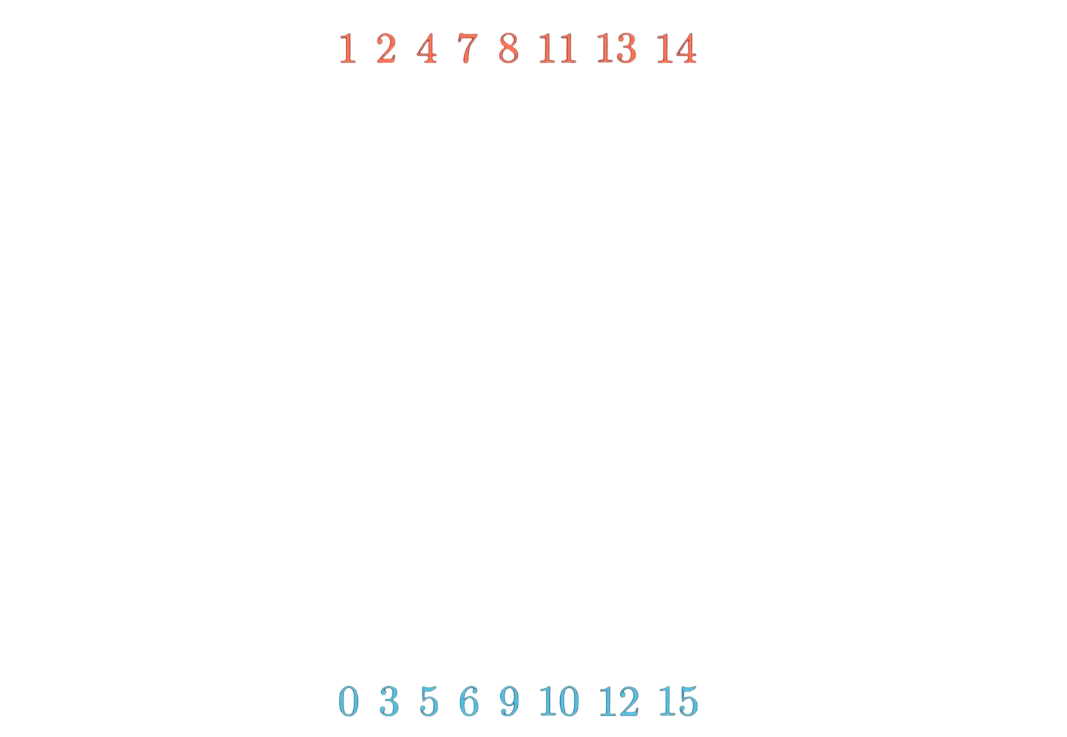
\includegraphics[width=\paperwidth]{FIRST.png}}
\end{frame}

\begin{frame}
    \makebox[\textwidth]{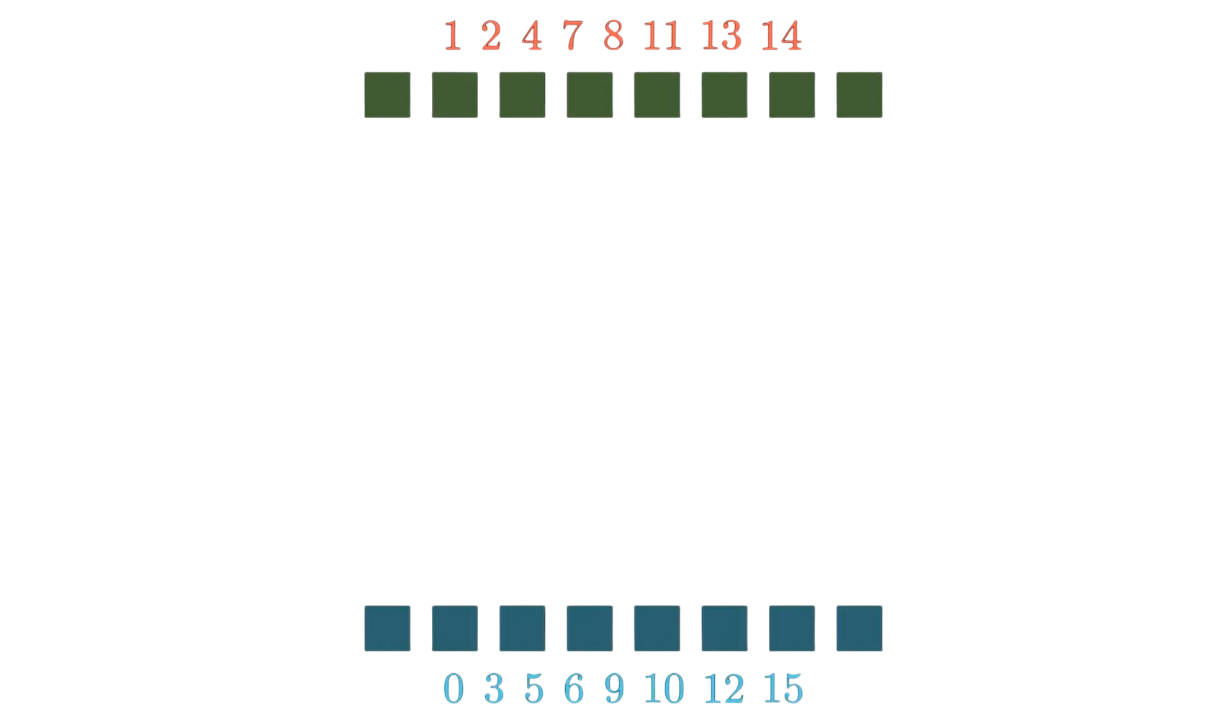
\includegraphics[width=\paperwidth]{0FIRST.png}}
\end{frame}

\begin{frame}
     \makebox[\textwidth]{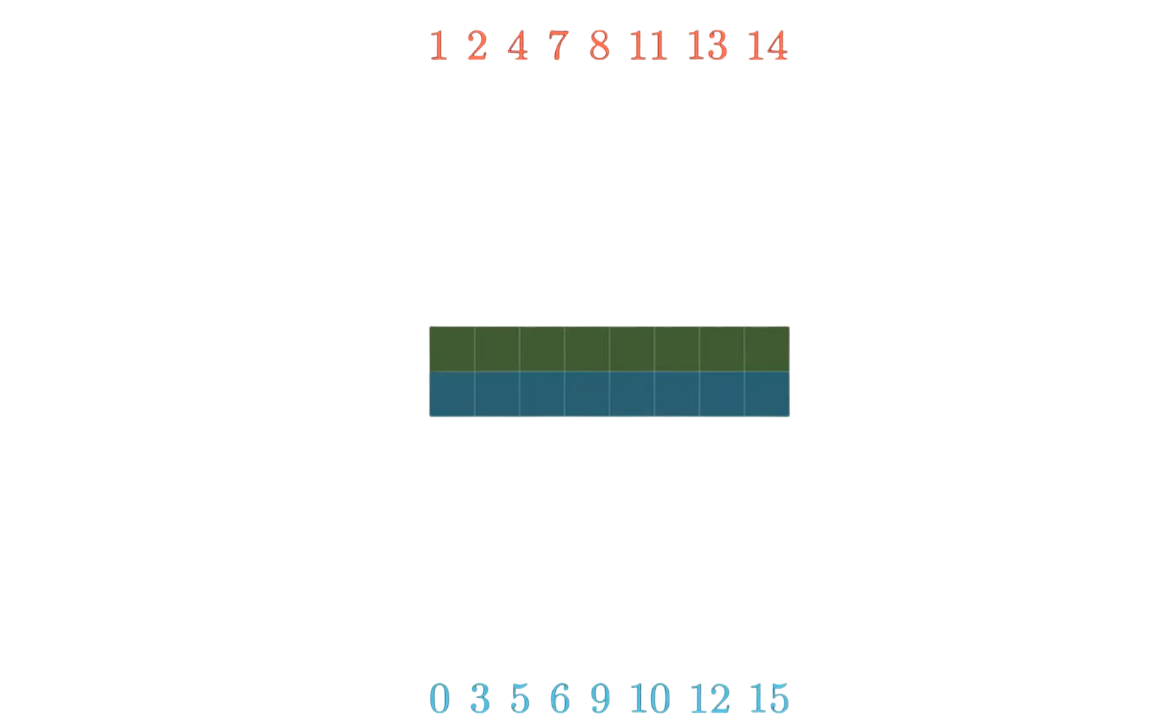
\includegraphics[width=\paperwidth]{0NEXT.png}}
\end{frame}

\begin{frame}
    \makebox[\textwidth]{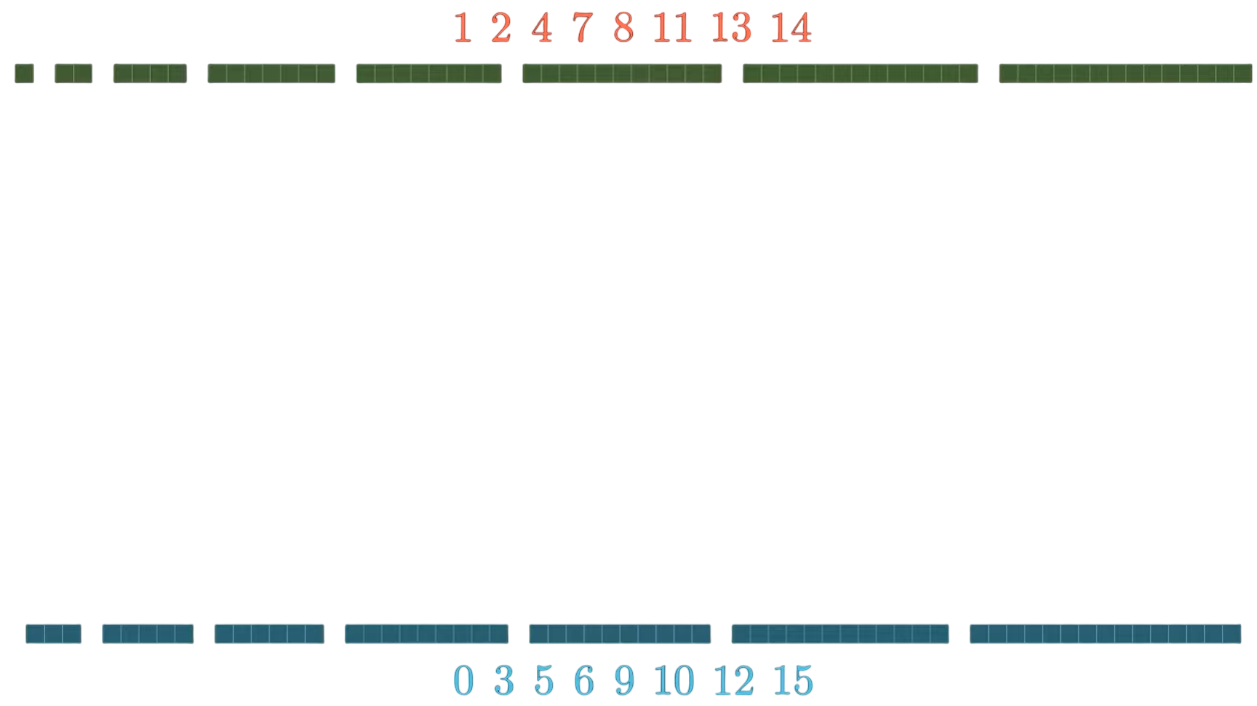
\includegraphics[width=\paperwidth]{1FIRST.png}}
\end{frame}

\begin{frame}
    \makebox[\textwidth]{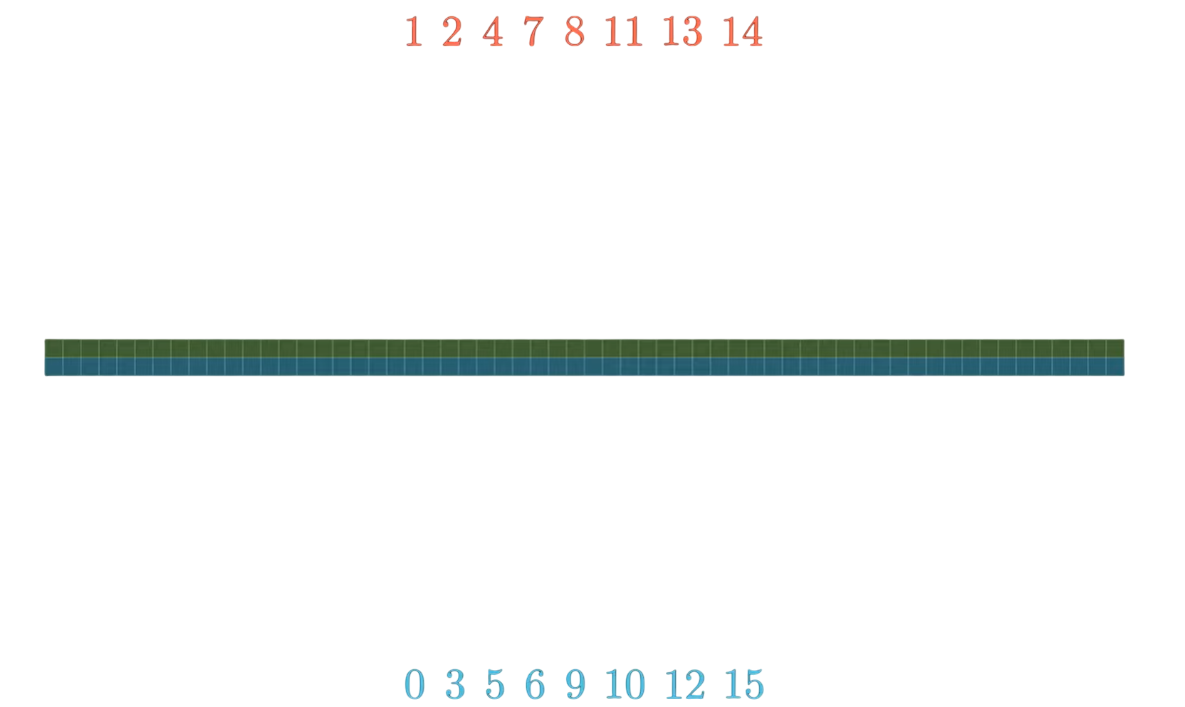
\includegraphics[width=\paperwidth]{1SECOND.png}}
\end{frame}

\begin{frame}
    \makebox[\textwidth]{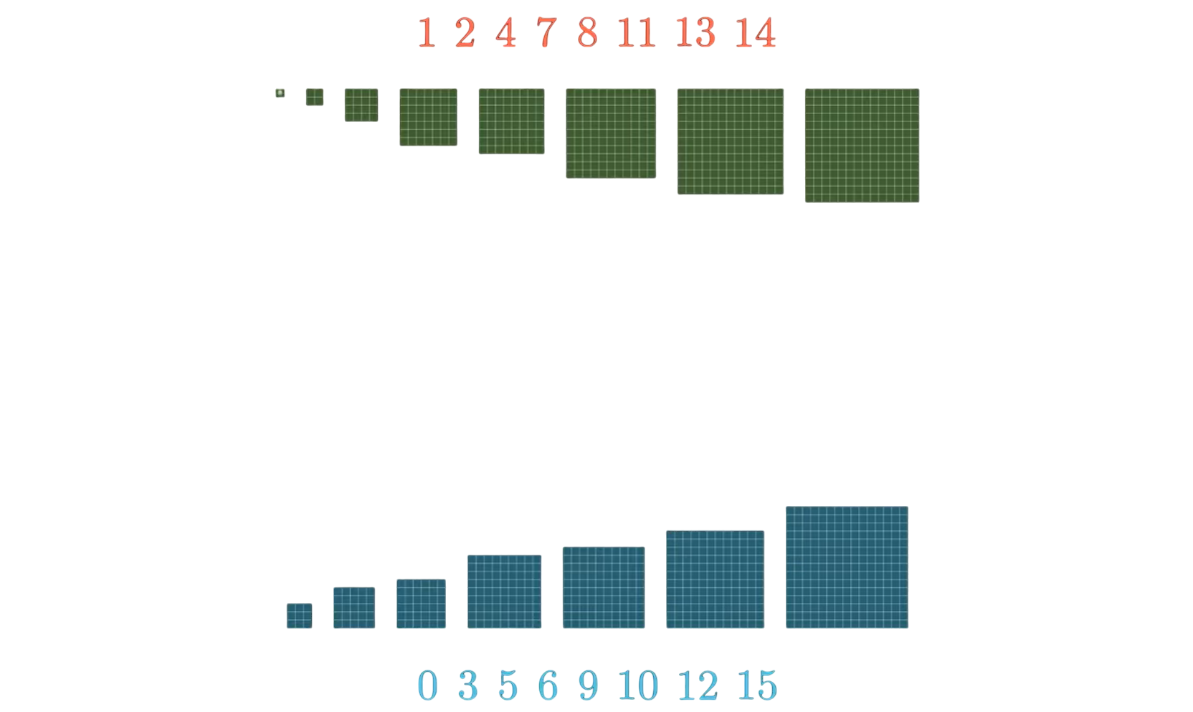
\includegraphics[width=\paperwidth]{2FIRST.png}}
\end{frame}

\begin{frame}
     \makebox[\textwidth]{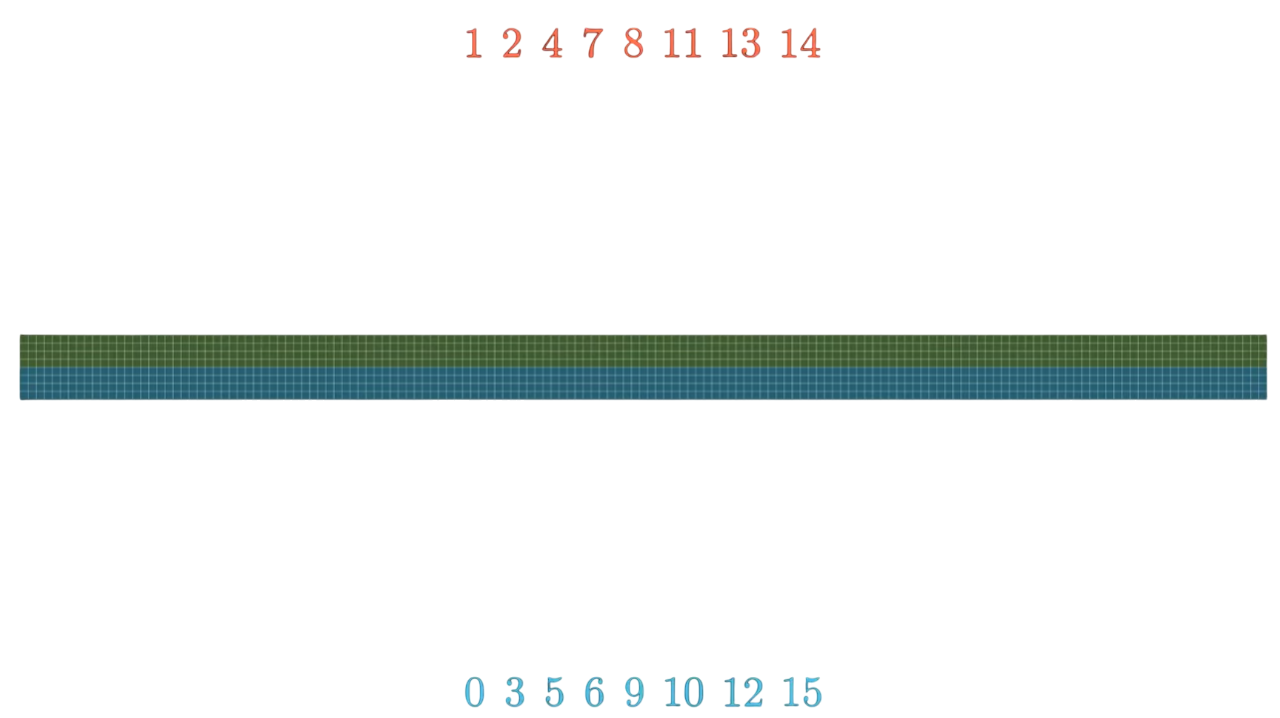
\includegraphics[width=\paperwidth]{2SECOND.png}}
\end{frame}

\begin{frame}

    % Group 1 numbers as a header at the top with spacing in red
    \begin{center}
    \textcolor{red}{\textbf{1 \hspace{0.5cm} 2 \hspace{0.5cm} 4 \hspace{0.5cm} 7 \hspace{0.5cm} 8 \hspace{0.5cm} 10 \hspace{0.5cm} 13 \hspace{0.5cm} 14}}
    \end{center}
    \vspace{1cm}

    \begin{center}
    $0^0 + 3^0 + 5^0 + 6^0 + 9^0 + 10^0 + 12^0 + 15^0 = 1^0 + 2^0 + 4^0 + 7^0 + 8^0 + 11^0 + 13^0 + 14^0$ \\
    $0^1 + 3^1 + 5^1 + 6^1 + 9^1 + 10^1 + 12^1 + 15^1 = 1^1 + 2^1 + 4^1 + 7^1 + 8^1 + 11^1 + 13^1 + 14^1$ \\
    $0^2 + 3^2 + 5^2 + 6^2 + 9^2 + 10^2 + 12^2 + 15^2 = 1^2 + 2^2 + 4^2 + 7^2 + 8^2 + 11^2 + 13^2 + 14^2$ \\
    $0^3 + 3^3 + 5^3 + 6^3 + 9^3 + 10^3 + 12^3 + 15^3 = 1^3 + 2^3 + 4^3 + 7^3 + 8^3 + 11^3 + 13^3 + 14^3$
    \end{center}

    
    \vfill % Pushes the remaining content downward
    
    % Group 0 numbers positioned below with spacing in blue
    \begin{center}
    \textcolor{blue}{\textbf{0 \hspace{0.5cm} 3 \hspace{0.5cm} 5 \hspace{0.5cm} 6 \hspace{0.5cm} 9 \hspace{0.5cm} 11 \hspace{0.5cm} 12 \hspace{0.5cm} 15}}
    \end{center}

\end{frame}

\begin{frame}
    \begin{theorem}
        The Thue-Morse sequence \( t = (t_n)_{n \geq 0} \) has the following property.  \\
        Define  
        
        \[I = \{0 \leq i < 2^N \mid t_i = 0\}\]
        
        \[J = \{0 \leq j < 2^N \mid t_j = 1\}\]
        
        Then for \( 0 \leq k < N \) we have  
        \[\sum_{i \in I} i^k = \sum_{j \in J} j^k.\]
    \end{theorem}
    
\end{frame}

\section{Math Problem}

\begin{frame}{Math Problem}
    There are many other interesting occurrences of this sequence but let's see one in mathematics.

    \vspace{1cm}
    
    \[
    \left(\frac{1}{2}\right)\left(\frac{3}{4}\right)\left(\frac{5}{6}\right) \left(\frac{7}{8}\right)\left(\frac{9}{10}\right)\left(\frac{11}{12}\right)\left(\frac{13}{14}\right)\dots \to 0
    \]

    \[
    \left(\frac{2}{1}\right)\left(\frac{4}{3}\right)\left(\frac{6}{5}\right) \left(\frac{8}{7}\right)\left(\frac{10}{9}\right)\left(\frac{12}{11}\right)\left(\frac{14}{13}\right)\dots \to \infty
    \]

\end{frame}

\begin{frame}{Math Problem}

    \[
    \begin{aligned}
        &\left(\frac{1}{2}\right) \quad \left(\frac{3}{4}\right) \quad \left(\frac{5}{6}\right) \quad \left(\frac{7}{8}\right) \quad \left(\frac{9}{10}\right) \quad \left(\frac{11}{12}\right) \quad \left(\frac{13}{14}\right) \quad \left(\frac{15}{16}\right) \dots \\
        &\quad 0 \quad \quad \:\:\:\, 1 \,\quad \quad \, \, \, \, \,1 \quad \quad \, \, \, \,\, 0 \quad \quad \quad  1 \quad \qquad \; \,0 \qquad \quad \,\,0 \qquad \quad \, \,  1
    \end{aligned}
    \]
    
    \[
    \begin{aligned}
        &\left(\frac{1}{2}\right) \quad \left(\frac{\textcolor{red}{4}}{\textcolor{red}{3}}\right) \quad \left(\frac{\textcolor{red}{6}}{\textcolor{red}{5}}\right) \quad \left(\frac{7}{8}\right) \quad \left(\frac{\textcolor{red}{10}}{\textcolor{red}{9}}\right) \quad \left(\frac{11}{12}\right) \quad \left(\frac{13}{14}\right) \quad \left(\frac{\textcolor{red}{16}}{\textcolor{red}{15}}\right) \dots \\
        &\quad 0 \quad \quad \:\:\:\, \textcolor{red}{1} \,\quad \quad \, \, \, \, \,\textcolor{red}{1} \quad \quad \, \, \, \,\, 0 \quad \quad \quad  \textcolor{red}{1} \quad \qquad \; \,0 \qquad \quad \,\,0 \qquad \quad \, \,  \textcolor{red}{1}
    \end{aligned}
    \]

\end{frame}

\begin{frame}{Math Problem}

\scriptsize

    \begin{theorem}
        If \( \varepsilon_n = (-1)^{t_n} \), then:
        \[
        \prod_{n=0}^\infty \left(\frac{2n+1}{2n+2}\right)^{\varepsilon_n} = \frac{\sqrt{2}}{2}
        \]
    \end{theorem}
    
    \textbf{Proof. Define: P and Q as follows:}
    \[
    P = \prod_{n=0}^\infty \left(\frac{2n+1}{2n+2}\right)^{\varepsilon_n},
    \quad
    Q = \prod_{n=1}^\infty \left(\frac{2n}{2n+1}\right)^{\varepsilon_n}
    \]
    
    Now, consider the product \(PQ\):
    \[
    PQ = \prod_{n=0}^\infty \left(\frac{2n+1}{2n+2}\right)^{\varepsilon_n} \cdot \prod_{n=1}^\infty \left(\frac{2n}{2n+1}\right)^{\varepsilon_n}
    \]

\end{frame}


\begin{frame}{Math Problem}
    \scriptsize
    
    We can replace this with the infinite product from $n=1$ to $\infty$ of the two expressions $P$ and $Q$ multiplied together, where we leave the $\frac{1}{2}$ out in front from the $n=0$ term of the product for $P$. 
    
    \[
        PQ = \frac{1}{2} \prod_{n=1}^\infty \left(\frac{2n+1}{2n+2} \cdot \frac{2n}{2n+1}\right)^{\varepsilon_n}.
    \]
    
    \[
        PQ = \frac{1}{2} \prod_{n=1}^\infty \left(\frac{n}{n+1}\right)^{\varepsilon_n}
    \]

    Now we break this infinite product into separate products over odd
    and even indices, we find :


    \[
        PQ = \frac{1}{2} \prod_{n=1}^\infty \left(\frac{n}{n+1}\right)^{\varepsilon_n} = \frac{1}{2} \prod_{n=1}^\infty \left(\frac{2n}{2n+1}\right)^{\textcolor{red}{\varepsilon_{2n}}} \cdot \prod_{n=0}^\infty \left(\frac{2n+1}{2n+2}\right)^{\textcolor{red}{\varepsilon_{2n+1}}}
    \]

    \[
        \textcolor{red}{\epsilon_{2n} = (-1)^{t_{2n}} = (-1)^{t_n} = \epsilon_n} 
        \hspace{1cm} 
        \textcolor{red}{\epsilon_{2n+1} = (-1)^{t_{2n+1}} = (-1)^{1-t_n} = -\epsilon_n}
    \]

    \[
        PQ = \frac{1}{2} \prod_{n=1}^\infty \left(\frac{2n}{2n+1}\right)^{\textcolor{red}{\varepsilon_{n}}} \cdot \prod_{n=0}^\infty \left(\frac{2n+1}{2n+2}\right)^{\textcolor{red}{-\varepsilon_{n}}} = \frac{1}{2} \prod_{n=1}^\infty \left(\frac{2n}{2n+1}\right)^{\textcolor{red}{\varepsilon_{n}}} \cdot \left(\prod_{n=0}^\infty \left(\frac{2n+1}{2n+2}\right)^{\textcolor{red}{\varepsilon_{n}}}\right)^{-1} = \frac{1}{2} \frac{Q}{P}
    \]

    \[
        PQ = \frac{1}{2} \frac{Q}{P} \rightarrow P^2 = \frac{1}{2} \rightarrow P = \sqrt{\frac{1}{2}} = \frac{\sqrt{2}}{2} 
        \hspace{1cm} 
        \boxed{Q = ?} \hspace{0.1cm} \boxed{\parbox{4.8cm}{ONE \textbf{COVRILUCA} FOR THOSE WHO CAN GIVE ME THE ANSWER}}
    \]
    
\end{frame}


\section{Fair Share Sequence}

\begin{frame}{Fair Share Sequence}
    \centering
    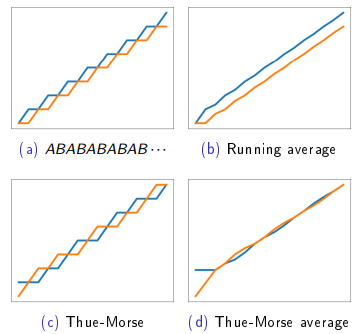
\includegraphics[height=0.8\textheight]{Thue.png}
\end{frame}

\begin{frame}[t]{Fair Share Sequence}
    \vspace{30px}
    Darius and Mihai are dividing things of non-increasing value amongst
    themselves. What is the fairest order for them to pick?
\end{frame}

\begin{frame}[t]{Fair Share Sequence}
    \vspace{30pt} 
    
    Darius and Mihai are dividing things of non-increasing value amongst
    themselves. What is the fairest order for them to pick?

    \medskip
    
    Suppose Darius picks first. Then Mihai should pick second, then Darius picks
    third, Mihai picks fourth, etc:

    \medskip
    
    \begin{center}
        DMDMDMDMDM \dots
    \end{center}
\end{frame}

\begin{frame}[t]{Fair Share Sequence}
    \vspace{30pt} 
    
    Darius and Mihai are dividing things of non-increasing value amongst
    themselves. What is the fairest order for them to pick?

    \medskip 
    
    Suppose Darius picks first. Then Mihai should pick second, then Darius picks
    third, Mihai picks fourth, etc:

    \medskip
    
    \begin{center}
        DMDMDMDMDM \dots
    \end{center}

    \medskip

    Darius gets an advantage: For every pair of items, Darius will get to pick
    the better one!

\end{frame}

\begin{frame}[t]{Fair Share Sequence}
    \vspace{30pt}
    Maybe after DM, what if they swapped order after?
    \begin{center}
        DM MD
    \end{center}

\end{frame}

\begin{frame}[t]{Fair Share Sequence}
    \vspace{30pt}
    Maybe after DM, what if they swapped order after?
    \begin{center}
        DM MD
    \end{center}

    \medskip
    
    Now it's more fair if there are 4 items, but if we repeat this:

    \begin{center}
        DMMD DMMD DMMD DMMD \dots
    \end{center}

\end{frame}

\begin{frame}[t]{Fair Share Sequence}
    \vspace{30pt}
    Maybe after DM, what if they swapped order after?
    \begin{center}
        DM MD
    \end{center}

    \medskip
    
    Now it's more fair if there are 4 items, but if we repeat this:

    \begin{center}
        DMMD DMMD DMMD DMMD \dots
    \end{center}

    \medskip

    Darius gets an advantage again: Darius will get to pick the best item out
    of every 4 items!


\end{frame}

\begin{frame}[t]{Fair Share Sequence}
    \vspace{30pt}
    Let's flip the order again:

    \begin{center}
        DMMD MDDM
    \end{center}

\end{frame}

\begin{frame}[t]{Fair Share Sequence}
    \vspace{30pt}
    Let's flip the order again:

    \begin{center}
        DMMD MDDM
    \end{center}

    \medskip
    
    Again, if we repeat this, Darius will get to pick the best item out of every 8 items!

\end{frame}

\begin{frame}[t]{Fair Share Sequence}
    \vspace{30pt}
    Let's flip the order again:

    \begin{center}
        DMMD MDDM
    \end{center}

    \medskip
    
    Again, if we repeat this, Darius will get to pick the best item out of every 8 items!

    \medskip

    If we keep flipping the order,

    \begin{center}
        DMMD MDDM MDDM DMMD MDDM DMMD DMMD MDDM \dots
    \end{center}

    If we replace D → 0 and M → 1, this is the Thue-Morse sequence!

\end{frame}

\section{Magic Squares}

\begin{frame}{Magic Squares}
    By a magic square of order T, we mean a T by T matrix whose entries are taken from the numbers 1, 2, 3, \dots ,$T^2$, and such that the sum of the entries in any row, column, or diagonal is the same number.

    One also requires that each of the numbers 1,2,3, \dots , $T^2$ be used exactly once as an entry.

    \begin{example}
        \begin{center}
            \setlength{\arrayrulewidth}{1pt} 
            \setlength{\tabcolsep}{0pt}
            \renewcommand{\arraystretch}{1.5}
            
            \begin{tabular}{|*{4}{>{\centering\arraybackslash}m{1.5cm}|}}
            \hline
            16 & 3  & 2  & 13 \\ \hline
            5  & 10 & 11 & 8  \\ \hline
            9  & 6  & 7  & 12 \\ \hline
            4  & 15 & 14 & 1  \\ \hline
            \end{tabular}
        \end{center}
    \end{example}
\end{frame}

\begin{frame}{Construction of magic squares of order T = $2^M$ with special properties using Thue-Morse Sequence}
    \scriptsize
    \small
    
    We illustrate this by constructing a 4 × 4 magic square, i.e. putting M = 2:

    \[
    \begin{array}{r*{16}{c}}
    & 1 & \textcolor{red}{2} & \textcolor{red}{3} & 4 & \textcolor{red}{5} & 6 & 7 & \textcolor{red}{8} & \textcolor{red}{9} & 10 & 11 & \textcolor{red}{12} & 13 & \textcolor{red}{14} & \textcolor{red}{15} & 16 \\
    t = & 0 & 1 & 1 & 0 & 1 & 0 & 0 & 1 & 1 & 0 & 0 & 1 & 0 & 1 & 1 & 0 \\
        & t_0 & t_1 & t_2 & t_3 & t_4 & t_5 & t_6 & t_7 & t_8 & t_9 & t_{10} & t_{11} & t_{12} & t_{13} & t_{14} & t_{15} \\
    \end{array}
    \]

    \begin{center}
        \setlength{\tabcolsep}{6pt}
        \renewcommand{\arraystretch}{2.3} 
        \begin{tabular}{|*{4}{>{\centering\arraybackslash}m{1.2cm}|}}
            \hline
            16 & \textcolor{red}{2}  & \textcolor{red}{3}  & 13 \\ \hline
            \textcolor{red}{5}  & 11 & 10 & \textcolor{red}{8}  \\ \hline
            \textcolor{red}{9}  & 7  & 6  & \textcolor{red}{12} \\ \hline
            4  & \textcolor{red}{14} & \textcolor{red}{15} & 1  \\ \hline
        \end{tabular}
    \end{center}

    \begin{center}
        \scriptsize
        \textbf{The n-th box of the magix square is n if $t_{n-1}$ = 1. The unused numbers are inserted in decreasing order into the empty boxes}
    \end{center}

\end{frame}

\begin{frame}{Magic Square}
    \begin{block}{Remark}
        The sum of the entries in any row, column or diagonal of a magic square of order T is \\
        \begin{center}
            $\frac{1}{2} T (T^2 + 1)$
        \end{center}
    \end{block}

    \begin{block}{Facts}
        \begin{enumerate}
        \small
        
            \item It is known that one can construct magic squares of any order except 2.
            
            \item Any magic square can be rotated and reflected to produce 8 trivially distinct squares, and the eight such squares are said to make up a single equivalence class.
            
            \item There is exactly one $3 \times 3$ magic square, exactly 880 $4 \times 4$ magic squares and exactly 275,305,224 $5 \times 5$ magic squares.
    \end{enumerate}
    \end{block}
\end{frame}

\section{Pattern Avoidance}

\begin{frame}{Pattern Avoidance}
    
    An \textcolor{red}{overlap} is a string of the form axaxa where a is a single letter and x is a string. 

    \vspace{0.3cm}

    Pick a binary word \( w \), such as \( w = 1101 \).
    
    \vspace{0.3cm}
    
    Consider blocks of the form \( 0w0w0 \) and \( 1w1w1 \).
    
    \vspace{0.3cm}
    
    Neither block appears ( no matter which \( w \) is chosen ).
    
    \vspace{0.3cm}
    
    The Thue-Morse Sequence is \textit{overlap free}.

    \vspace{0.7cm}

    \[
    \begin{aligned}
        &011010011001011010010110011010011001011001101001011010\dots \\ 
        &\textcolor{red}{0}\textcolor{forestgreen}{1101}\textcolor{red}{0}\textcolor{forestgreen}{1101}\textcolor{red}{0} \\ 
        &\textcolor{cyan}{1}\textcolor{forestgreen}{1101}\textcolor{cyan}{1}\textcolor{forestgreen}{1101}\textcolor{cyan}{1}
    \end{aligned}
\]
 
\end{frame}

\begin{frame}{Pattern Avoidance}

    Count the numbers of 1s between succesive 0s.
    
    \[
    \begin{aligned}
        &\textcolor{red}{0}11\textcolor{red}{0}10011001011010010110011010011001011001101001011010\dots \\ 
        &2
    \end{aligned}
    \]
 
\end{frame}

\begin{frame}{Pattern Avoidance}

    Count the numbers of 1s between succesive 0s.
    
    \[
    \begin{aligned}
        &011\textcolor{red}{0}1\textcolor{red}{0}011001011010010110011010011001011001101001011010\dots \\ 
        &21
    \end{aligned}
    \]
 
\end{frame}

\begin{frame}{Pattern Avoidance}

    Count the numbers of 1s between succesive 0s.
    
    \[
    \begin{aligned}
        &01101\textcolor{red}{0}\textcolor{red}{0}11001011010010110011010011001011001101001011010\dots \\ 
        &210
    \end{aligned}
    \]
 
\end{frame}

\begin{frame}{Pattern Avoidance}

    Count the numbers of 1s between succesive 0s.
    
    \[
    \begin{aligned}
        &011010\textcolor{red}{0}11\textcolor{red}{0}01011010010110011010011001011001101001011010\dots \\ 
        &2102
    \end{aligned}
    \]
 
\end{frame}

\begin{frame}{Pattern Avoidance}

    We keep doing this counting the number of 1s between the next two successive 0s until we get an infinite integer sequence made of 2s, 1s and 0s like this one :
    
    \[
    \begin{aligned}
        &210201210120210201202102012021012102012102012102012\dots
    \end{aligned}
    \]
    A \textcolor{red}{square} is a string of the form xx.\\
    A word is \textcolor{red}{squarefree} if it contains no subword (block of consecutive symbols) that is a square. Note that \textcolor{red}{squarefree} is not squarefree, but \textcolor{red}{square} is.

    Consider any ternary (base 3) word $w$ such as  $w$ = 01212. If we look through the entire sequence to see if we can find this block $0121201212$ it turns out that no matter which $w$ we choose the repeated block pattern $ww$ will never appear. This new squence is called \textit{square free}.

    \[
    \begin{aligned}
        &210201210120210201202102012021012102012102012102012\dots \\
        &\textcolor{red}{0121201212}
    \end{aligned}
    \]
 
\end{frame}

\section{Music}

\begin{frame}{Music}

    Thue-Morse Sequence has even been used to composing music! 

    \vspace{0.5cm}

    Tom Johnson, a Paris-based composer, has used the Thue-Morse
    sequence and other sequences formed by iterated morphisms, in his
    work.

    \vspace{0.5cm}

    \begin{center}
    
    \makebox[\textwidth]{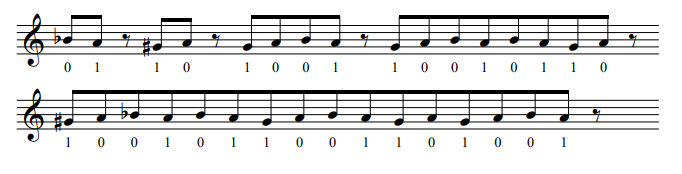
\includegraphics[width=\textwidth]{music.png}}
    \vspace{0.5em}
    \textcolor{blue}{Figure:} Composition by Tom Johnson

    \end{center}
    
\end{frame}

%%%%%%%%%

\section{An interesting problem}

\begin{frame}{Twenty Questions with a liar}
    Consider a game in which one player chooses an integer \( x \in [1, 1000] \), and the other player has to guess it by asking yes/no questions. The second player is allowed to give at most one incorrect answer.
    \newline
    
    What is the minimum number of yes/no questions required to guarantee the identification of the chosen number?
    \newline

    30\dots 27\dots 21\dots who says lower? Place your bets!
\end{frame}

\begin{frame}{Twenty Questions with a liar - Solution}
    Let us denote the bits of the first player's number by $a_i$, where $i \in [1..10]$. We start by asking the values of all those bits. That is, we ask the following questions: "Is it true that the $i$ th bit of your number is zero?" Let us denote the answers to these questions as $b_i$, where $i \in [1..10]$.

    \vspace{1cm}

    \centering
    \begin{tabular}{cccccccccc}
        \rule{0.5cm}{1.5pt} & \rule{0.5cm}{1.5pt} & \rule{0.5cm}{1.5pt} & \rule{0.5cm}{1.5pt} & \rule{0.5cm}{1.5pt} & \rule{0.5cm}{1.5pt} & \rule{0.5cm}{1.5pt} & \rule{0.5cm}{1.5pt} & \rule{0.5cm}{1.5pt} & \rule{0.5cm}{1.5pt} \\
        $a_{10}$ & $a_9$ & $a_8$ & $a_7$ & $a_6$ & $a_5$ & $a_4$ & $a_3$ & $a_2$ & $a_1$
    \end{tabular}

    \vspace{1cm}

    \centering
    \begin{tabular}{cccccccccc}
        \rule{0.5cm}{1.5pt} & \rule{0.5cm}{1.5pt} & \rule{0.5cm}{1.5pt} & \rule{0.5cm}{1.5pt} & \rule{0.5cm}{1.5pt} & \rule{0.5cm}{1.5pt} & \rule{0.5cm}{1.5pt} & \rule{0.5cm}{1.5pt} & \rule{0.5cm}{1.5pt} & \rule{0.5cm}{1.5pt} \\
        $b_{10}$ & $b_9$ & $b_8$ & $b_7$ & $b_6$ & $b_5$ & $b_4$ & $b_3$ & $b_2$ & $b_1$
    \end{tabular}
\end{frame}


\begin{frame}{Twenty Questions with a liar - Solution}
    Now, we ask 4 additional questions: \begin{itemize}
        \item Is it true that $a_1 \oplus a_2 \oplus a_4 \oplus a_5 \oplus a_7 \oplus a_9 = 0$? ($\oplus$ denotes summation modulo 2.)
        \item Is it true that $a_1 \oplus a_3 \oplus a_4 \oplus a_6 \oplus a_7 \oplus a_{10} = 0$?
        \item Is it true that $a_2 \oplus a_3 \oplus a_4 \oplus a_8 \oplus a_9 \oplus a_{10} = 0$?
        \item Is it true that $a_5 \oplus a_6 \oplus a_7 \oplus a_8 \oplus a_9 \oplus a_{10} = 0$?
    \end{itemize}
\end{frame}

\begin{frame}{Twenty Questions with a liar - Solution}
    Let $q_1$, $q_2$, $q_3$, and $q_4$ be the answers to these additional questions. Now, the second player calculates $t_i$ for $i \in [1..4]$ --- answers to those questions based on the bits $b_j$ which he previously received from the first player.

    There are 16 ways in which the bits $q_i$ can differ from $t_i$. Let $d_i = q_i \oplus t_i$ (thus $d_i = 1$ if and only if $q_i \neq t_i$).
\end{frame}

\begin{frame}{Twenty Questions with a liar - Solution}
    \scriptsize
    \centering
    Let us now construct a table of all possible errors and corresponding values of $(d_1, d_2, d_3, d_4)$:
    
    \vspace{1em}

    \begin{tabular}{cc}
        \begin{tabular}{|c|c|}
            \hline
            \textbf{Error in} & $(d_1,d_2,d_3,d_4)$ \\
            \hline
            No error & (0,0,0,0) \\
            $b_1$ & (1,1,0,0) \\
            $b_2$ & (1,0,1,0) \\
            $b_3$ & (0,1,1,0) \\
            $b_4$ & (1,1,1,0) \\
            $b_5$ & (1,0,0,1) \\
            $b_6$ & (0,1,0,1) \\
            $b_7$ & (1,1,0,1) \\
            $b_8$ & (0,0,1,1) \\
            $b_9$ & (1,0,1,1) \\
            $b_{10}$ & (0,1,1,1) \\
            \hline
        \end{tabular}
        &
        \begin{tabular}{|c|c|}
            \hline
            \textbf{Error in} & $(d_1,d_2,d_3,d_4)$ \\
            \hline
            $q_1$ & (1,0,0,0) \\
            $q_2$ & (0,1,0,0) \\
            $q_3$ & (0,0,1,0) \\
            $q_4$ & (0,0,0,1) \\
            \hline
        \end{tabular}
    \end{tabular}

    \vspace{1em}
    All values of $(d_1,d_2,d_3,d_4)$ are distinct, so the error can be identified and corrected.
\end{frame}

\end{document}
